% Drawing 74/05-5 -- folder 74, batch 05, archive page 82 (PDF page 83).
% Transcription: Grand diagramme écrit en travers de la page (feuille tournée), reliant des ensembles d'hexagones : $\mathrm{Hex}_{s}\simeq\mathrm{hex}$ ($\simeq$ tria), $\mathrm{Hex}_{\mathrm{tr}}$ ($\simeq$ \ill{} tria), $\mathrm{Hex}_{s*}$, $\mathrm{Hex}_{\mathrm{tr}*}$ (triplets de \ill{}), $\mathrm{Hex}_{\mathrm{ép}}$, $\mathrm{Hex}_{\mathrm{tri}}$, $\mathrm{Hex}_{d}$ ($\simeq$ tria \ill{}), $\mathrm{Hex}$ ($\simeq$ pav) et « tri hex », par des flèches horizontales marquées $3$ et des flèches verticales et obliques marquées $2$, formant un réseau en forme de prisme.
% Kind: prism-shaped arrow diagram (sheet turned). Method 2 (schematic redraw from the facsimile). Status: partial.
% Notes: Written across the page: the labels read bottom to top and are set with rotate=90 in the TikZ, at \small (the figure drawn at 1.2 mm per unit). Nodes: Hex_s = hex (= tria), Hex_tr (= ... tria), Hex_s*, Hex_tr* (triplets de ...), Hex_ép and Hex_tri (top), Hex_d (= tria ...), Hex (= pav) and tri hex (bottom row). Horizontal arrows marked 3 (Hex_s -> Hex_tr, Hex_s* -> Hex_tr*, Hex_ép -> Hex_tri, Hex_d -> Hex, Hex -> tri hex, the last bold), vertical ones marked 2 (Hex_s -> Hex_d, Hex_tr -> Hex, Hex_tri -> Hex_tr*, and the stroke Hex_ép - Hex_s*), oblique ones marked 2 (Hex_ép -> Hex_s, Hex_tri -> Hex_tr, Hex_s* -> Hex_d, Hex_tr* -> Hex), as on the page. Still differs: the illegible parts of the side labels are left out (as \dots); the stroke from Hex_ép down to Hex_s* has no visible head. Nothing is struck. The text lines above and below are text. Redrawn 2026-11-09 (issue 128): to check again. Overlay check 2026-11-13 (issue 147, Claude claude-opus-5-5): the redraw, rasterised by the skill's previewer (not compiled: no TeX in the session), laid over the 300 dpi colour crop of the scan (261 ppi). The nodes (their labels turned with the sheet) and the arrows lie on their ink to within 1 to 3 units. Still differs, as said above: the illegible parts of the side labels are left out, and the stroke from Hex_ép down to Hex_s* has no visible head. It is an arrow diagram, which the editor prefers set as LaTeX (tikz-cd or array) in the transcription; as a redraw it stays partial.
% Coordinates: 1 unit = 1.2 mm = 1/100 of the crop width (bbox in page fractions: [0.58, 0.58, 0.92, 0.88]).
% Redrawn by Claude (claude-opus-5-5), issue #73, 2026-11-09; not checked by a human; not compiled (no TeX in the session).
% Checked by Claude (claude-opus-5-5) 2026-11-13 (issue #147): overlaid on the 300 dpi colour facsimile; not compiled (no TeX in the session). Status: partial.
% Rights: reproduces part of the work -- behind RENDER_TRANSCRIPTS, never published by itself.
\documentclass[tikz,border=3pt]{standalone}
\usepackage{amsmath,amssymb}
\usetikzlibrary{patterns,arrows.meta}
\tikzset{pencil/.style={black!45}, struck/.style={black!35}, mark/.style={circle,draw,inner sep=1.3pt}, pt/.style={circle,fill,inner sep=0.9pt}, opt/.style={circle,draw,fill=white,inner sep=1.1pt}}
\begin{document}
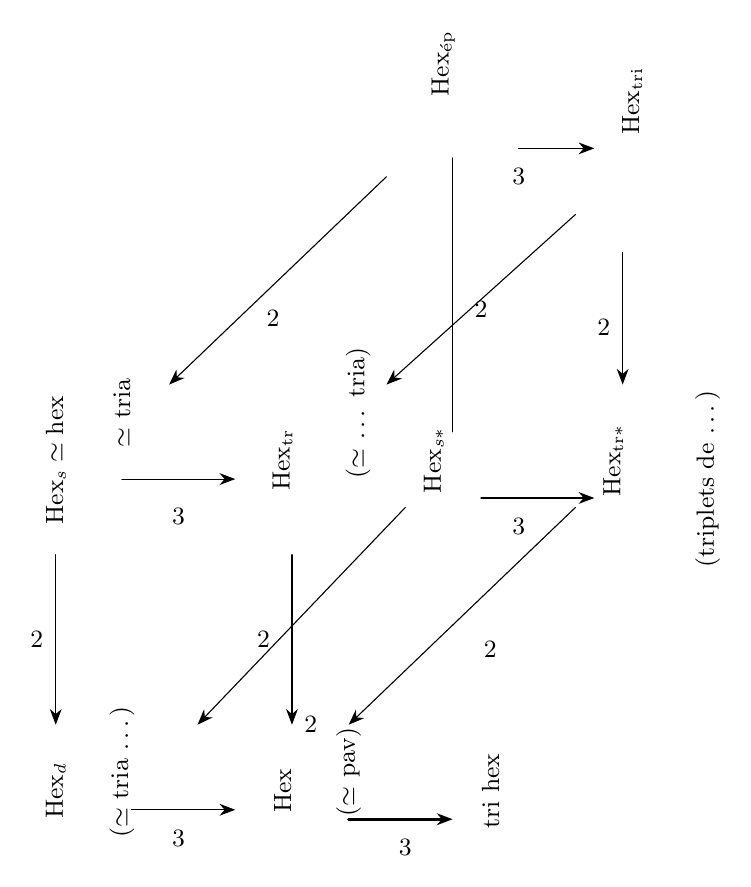
\begin{tikzpicture}[x=1.2mm,y=1.2mm,line cap=round,line join=round,font=\scriptsize]
\node[inner sep=1pt,rotate=90] at (13,-60) {\small $\mathrm{Hex}_s\simeq\mathrm{hex}$};
\node[inner sep=1pt,rotate=90] at (20,-55) {\small $\simeq$ tria};
\node[inner sep=1pt,rotate=90] at (37,-60) {\small $\mathrm{Hex}_{\mathrm{tr}}$};
\node[inner sep=1pt,rotate=90] at (45,-55) {\small ($\simeq$ \dots\ tria)};
\node[inner sep=1pt,rotate=90] at (53,-60) {\small $\mathrm{Hex}_{s*}$};
\node[inner sep=1pt,rotate=90] at (72,-60) {\small $\mathrm{Hex}_{\mathrm{tr}*}$};
\node[inner sep=1pt,rotate=90] at (82,-62) {\small (triplets de \dots)};
\node[inner sep=1pt,rotate=90] at (54,-18) {\small $\mathrm{Hex}_{\mathrm{\acute ep}}$};
\node[inner sep=1pt,rotate=90] at (74,-22) {\small $\mathrm{Hex}_{\mathrm{tri}}$};
\node[inner sep=1pt,rotate=90] at (13,-95) {\small $\mathrm{Hex}_d$};
\node[inner sep=1pt,rotate=90] at (20,-93) {\small ($\simeq$ tria \dots)};
\node[inner sep=1pt,rotate=90] at (37,-95) {\small $\mathrm{Hex}$};
\node[inner sep=1pt,rotate=90] at (44,-93) {\small ($\simeq$ pav)};
\node[inner sep=1pt,rotate=90] at (59,-95) {\small tri hex};
\draw[-{Stealth[length=2mm]}] (20,-62) -- (32,-62);
\node[inner sep=1pt] at (26,-66) {\small $3$};
\draw[-{Stealth[length=2mm]}] (58,-64) -- (70,-64);
\node[inner sep=1pt] at (62,-67) {\small $3$};
\draw[-{Stealth[length=2mm]}] (21,-97) -- (32,-97);
\node[inner sep=1pt] at (26,-100) {\small $3$};
\draw[-{Stealth[length=2mm]},very thick] (44,-98) -- (55,-98);
\node[inner sep=1pt] at (50,-101) {\small $3$};
\draw[-{Stealth[length=2mm]}] (62,-27) -- (70,-27);
\node[inner sep=1pt] at (62,-30) {\small $3$};
\draw[-{Stealth[length=2mm]}] (13,-70) -- (13,-88);
\node[inner sep=1pt] at (11,-79) {\small $2$};
\draw[-{Stealth[length=2mm]}] (38,-70) -- (38,-88);
\node[inner sep=1pt] at (40,-88) {\small $2$};
\draw (55,-28) -- (55,-57);
\draw[-{Stealth[length=2mm]}] (73,-38) -- (73,-52);
\node[inner sep=1pt] at (71,-46) {\small $2$};
\draw[-{Stealth[length=2mm]}] (48,-30) -- (25,-52);
\node[inner sep=1pt] at (36,-45) {\small $2$};
\draw[-{Stealth[length=2mm]}] (68,-34) -- (48,-52);
\node[inner sep=1pt] at (58,-44) {\small $2$};
\draw[-{Stealth[length=2mm]}] (50,-65) -- (28,-88);
\node[inner sep=1pt] at (35,-79) {\small $2$};
\draw[-{Stealth[length=2mm]}] (68,-65) -- (44,-88);
\node[inner sep=1pt] at (59,-80) {\small $2$};
\end{tikzpicture}
\end{document}
